\documentclass[12pt,journal,transmag]{IEEEtran}

\usepackage{cite}
\usepackage[pdftex]{graphicx}
% declare the path(s) where your graphic files are
\graphicspath{IMAGES/}
\DeclareGraphicsExtensions{.pdf,.jpeg,.png,.jpg}
\usepackage{amsmath}
\interdisplaylinepenalty=2500
\usepackage{algorithmic}
\usepackage{array}
\usepackage{booktabs}
\usepackage[caption=false,font=normalsize,labelfont=sf,textfon =sf]{subfig}
\usepackage{dblfloatfix}
\usepackage{url}
\usepackage{lipsum}
\usepackage{xcolor}
\usepackage{listings}
\usepackage[margin=1in]{geometry}
\usepackage{setspace}
\onehalfspacing


\lstset{
	escapeinside={/*@}{@*/},
	language=Java,	
	basicstyle=\fontsize{8.5}{12}\selectfont,
	numbers=left,
	numbersep=2pt,    
	xleftmargin=2pt,
	frame=tb,
	columns=fullflexible,
	showstringspaces=false,
	tabsize=4,
	keepspaces=true,
	showtabs=false,
	showspaces=false,
	morekeywords={inline,public,class,private,protected,struct},
	captionpos=b,
	lineskip=-0.4em,
	aboveskip=10pt,
	extendedchars=true,
	breaklines=true,
	prebreak = \raisebox{0ex}[0ex][0ex]{\ensuremath{\hookleftarrow}},
	keywordstyle=\color[rgb]{0,0,1},
	commentstyle=\color[rgb]{0.133,0.545,0.133},
	stringstyle=\color[rgb]{0.627,0.126,0.941},
}

% correct bad hyphenation here
\hyphenation{hy-phen}

\begin{document}
	
	\title{SET10108 Concurrent and Parallel Systems\\Report for Coursework Part 2}
	
	\author{\IEEEauthorblockN{Beej Persson, 40183743@live.napier.ac.uk}
		\IEEEauthorblockA{School of Computing,
			Edinburgh Napier University, Edinburgh}% <-this % stops an unwanted space
		
		\thanks{November 2017}}
	
	
	\markboth{40183743}{}
	% The only time the second header will appear is for the odd numbered pages after the title page when using the twoside option.
	
	\IEEEtitleabstractindextext{
		\begin{abstract}
			For part 2 of the coursework required for the SET10108 Concurrent and Parallel Systems module at Edinburgh Napier University an n-body simulation algorithm's performance was to be evaluated and improved by utilising parallel techniques. This report documents one such investigation where the algorithm was parallelised and the difference in its performance was measured. 
		\end{abstract}
		
		\begin{IEEEkeywords}
			parallel, n-body, OpenMP, CUDA, C++11, performance, speedup, efficiency.
		\end{IEEEkeywords}}
	
	\maketitle
	
	\IEEEdisplaynontitleabstractindextext
	
	\IEEEpeerreviewmaketitle
	
	\section{Introduction and Background}
	\IEEEPARstart{T}{he} aim of this report is to evaluate the performance of a ray tracing algorithm and attempt to improve this performance using parallel techniques. The ray tracer initially processes sequentially on a single core of the CPU, but by investigating different parallel techniques the algorithm was changed to run on multiple threads in an attempt to increase the performance.
	
	\subsection{Ray Tracer}
	Ray tracing is a technique used to render an image where "a ray is cast through every pixel of the image, tracing the light coming from that direction" \cite{ray}. The path is traced from an imaginary eye through each pixel on a virtual image plane and the colour of the object visible through it is calculated. It is typically capable of producing visually realistic images of high quality but at a greater computational cost compared to typical rendering techniques. Therefore it tends to be used when an image can be generated slowly ahead of time, but isn't so well suited to the real-time rendering requirements of video games.
	
	\section{Initial Analysis}
	The provided algorithm generates the image by iterating through each pixel using nested for loops. The ray tracer can also sample each pixel multiple times to produce a more accurate and detailed image but at the cost of processing time. Upon running the program a few times and changing the dimensions of the image produced and the number of samples per pixel an idea of its base-line performance was gathered.  By its nature of currently operating sequentially, increasing either the dimensions of the image produced or the number of samples per pixel increases the time it takes to produce the image with an almost perfect positive correlation. That is to say: doubling the size of the image produced or doubling the samples per pixel doubles the time taken.\\
	
	\lstinputlisting[caption = The many nested for loops of the ray tracer algorithm with the operations within the loops removed for clarity.]{./sourceCode/forloop.cpp}
	
	For smaller images at a low number of samples per pixel this results in reasonable times to produce an image, but when producing large images at a high number of samples per pixel the time to produce them was bottlenecked by only running sequentially on a single thread. Most of the time running the program is spent iterating through the nested for loops (seen in Listing 1) and so a clear solution to improving the performance of the algorithm is to run these for loops concurrently on multiple threads.
	
	
	\section{Methodology}	
	A systematic approach was undertaken to evaluate the performance of the algorithm and attempt to measure any improvements in performance gained by parallelising the algorithm.
	
	The first step was to run a series of tests on the provided sequential algorithm to provide a base-line that the performance of the different parallel techniques could be compared to. These tests were all done on the same hardware, the relevant specifications of which are shown in table \ref{hardware}. The details of the tests are shown in the testing subsection below.
	
	\begin{table}[!h]
		\renewcommand{\arraystretch}{1.3}
		\caption{Hardware Specifications}
		\label{hardware}
		\centering
		\begin{tabular}{|l|l|}
			\hline
			Processor & i7-4790K 4 Core HT @ 4.00GHz\\ \hline
			RAM & 16.0GB\\ \hline
			OS & Windows 10 Pro 64-bit\\ \hline
		\end{tabular}
	\end{table}
	
	\subsection{Parallelisation Techniques}
	After these benchmarks for the sequential algorithm were recorded, a few different parallelising techniques were applied to the algorithm and some preliminary tests were run. The intention here was to ensure that the techniques had been implemented correctly and to gain an idea of their relative performance. The techniques used were manual multi-threading and OpenMP with both static and dynamic scheduling.\\
	
	\subsubsection{Manual Multi-Threading}
	To parallelise the algorithm using manual multi-threading the set of for loops seen in Listing 1 were added to a single method which could then be run on multiple threads, as shown in Listing 2.
	
	\lstinputlisting[caption = The for loop used to run the forLoopAlgorithm method accross the required number of threads. The variables that are passed to the method are removed for clarity.]{./sourceCode/manualmulti-threading.cpp}
	
	\subsubsection{OpenMP}
	OpenMP is an API that supports shared-memory parallel programming and allows some additional manipulations in the scheduling that were used in an attempt to increase performance. The pre-processor argument shown in Listing 3 was used to parallelise the outer for loop, allowing the algorithm to be run across multiple threads.
	
	\lstinputlisting[caption = The OpenMP parallel for used to parallelise the shown for loop across the number of threads desired. The removed nested for loops can be seen in Listing 1.]{./sourceCode/omp.cpp}
	
	OpenMP's parallel for function comes with a \textit{schedule} clause, seen in Listing 3, that can be used to change the way it spreads the workload across the threads. By default, OpenMP statically assigns each for loop iteration to a thread. However, if each iteration takes a different amount of time, it can be beneficial to use dynamic scheduling. When scheduled dynamically the threads can request work when ready and be assigned the next iteration that hasn't been executed yet. Given that this may further improve the performance of the ray tracing algorithm, both types of scheduling were tested.
	
	\subsection{Testing}
	The same series of tests that were run on the sequential algorithm were then undertaken for each implemented parallelisation. These tests were done under the same conditions and on the same hardware to eliminate discrepancies. The testing parameters used to evaluate the performance of the algorithms is outlined below.
	
	For the majority of the tests, the algorithms were run on the maximum number of threads available (the test hardware allowed up to 8). The dependent variable being measured was the amount of time it took for the algorithms to produce all the data in the pixel vector, which is used to generate the final image. The independent variables were the dimensions of the image, the number of samples per pixel. First the image size was kept constant at 256x256 whilst the number of samples per pixel was incremented, by powers of 2, from 4 up to 512. After this the samples per pixel was kept constant at 16 whilst the dimensions of the image were incremented, again by powers of 2, from 128x128 up to 1024x1024. For each change in the independent variables, 100 tests were run and the time it took for the algorithm to produce the data recorded, before the average run times were calculated. Further to this, 2 tests were run with a large image size of 1024x1024 and 1024 samples per pixel. This was only done twice due to how long it took for the sequential algorithm to generate the image, but was still useful for comparison. Additionally a few tests were done on each parallel algorithm where the number of threads they ran on were controlled. This was done to help contextualise whether the potential performance increase came from the number of additional threads or from changes to the algorithm itself.
	
	\subsection{Evaluation}
	The results of these tests were then collated and compared to the results from the sequential algorithm's testing and used as the basis for the evaluation of	their respective performance.
	
	To represent the improved performance, the efficiency, $E$, of the algorithms was calculated using the formula shown in Equation \ref{efficiencyeq} below:
	
	\begin{equation} \label{efficiencyeq} 
	E = \dfrac{S}{p} = \dfrac{(\dfrac{T_{serial}}{T_{parallel}})}{p}
	\end{equation}
	
	Where $S$ is speedup, $p$ is the number of processor cores (the test hardware had 4), and $T_{serial}$ and $T_{parallel}$ are the sequential and parallel computational times respectively.
	
	\section{Results and Discussion}
	The results from the performance testing done on the algorithms can be seen summarised in tables \ref{comptable1} and \ref{comptable2} below. As discussed in the initial analysis there is an almost perfect positive correlation between the average time and the increasing samples per pixel and image dimensions for the sequential algorithm, but this also holds true for parallel algorithms. However, the times in which the parallel algorithms produced the data were much lower than the sequential algorithm, even at extreme values (Table \ref{comptable3}).
	
	Table \ref{comptable1} and its accompanying graph (Figure \ref{graph1}) comparing the average time taken for the algorithms to generate the data required to produce a 256x256 image at different numbers of samples per pixel are shown below.
	
	\begin{table}[!h]
		\caption{256x256 Image Generation Performance Comparison}
		\label{comptable1}
		\centering
		\resizebox{\columnwidth}{!}{%
			\begin{tabular}{@{}ccccc@{}}
				\toprule
				\multicolumn{5}{c}{Image Dimensions = 256x256} \\ \midrule
				\multicolumn{1}{c|}{Algorithm} & \multicolumn{1}{c}{Sequential} & \multicolumn{1}{c}{OMP Static} & \multicolumn{1}{c}{OMP Dynamic} & \multicolumn{1}{c}{Manual} \\ \midrule
				\multicolumn{1}{c|}{SamplesPerPixel} & \multicolumn{4}{c}{Average Time / ms} \\ \midrule
				\multicolumn{1}{c|}{4} & 762.57 & 187.13 & 163.98 & 168.87 \\
				\multicolumn{1}{c|}{8} & 1536.27 & 372.96 & 328.74 & 333.76 \\
				\multicolumn{1}{c|}{16} & 3059.91 & 728.10 & 655.39 &649.57 \\
				\multicolumn{1}{c|}{32} & 6223.33 & 1427.95 & 1308.69 & 1283.35 \\
				\multicolumn{1}{c|}{64} & 12510.68 & 2804.45 & 2625.94 & 2570.45 \\
				\multicolumn{1}{c|}{128} & 24544.85 & 5589.91 & 5206.20 & 5100.70 \\
				\multicolumn{1}{c|}{256} & 48129.36 & 11119.07 & 10354.04 & 10108.84 \\
				\multicolumn{1}{c|}{512} & 95256.72 & 22138.99 & 20634.72 & 20348.64 \\ \bottomrule
			\end{tabular}%
		}
	\end{table}
	
	\begin{figure*}[!h]
		\centering
		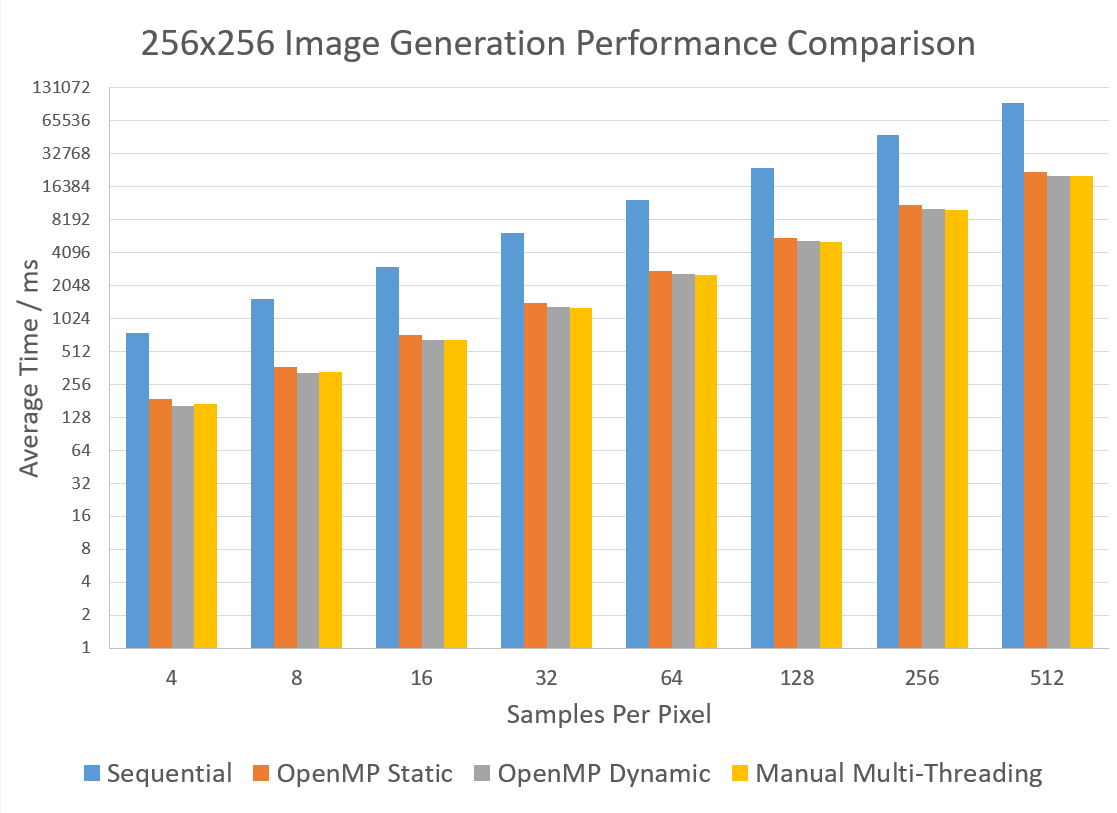
\includegraphics[width=\textwidth]{IMAGES/performancecomparison1}
		\caption{A graph showing the average time it took each algorithm to generate a 256x256 image at different numbers of samples per pixel.}
		\label{graph1}
	\end{figure*}
	
	As the number of samples per pixel were incremented in powers of 2, the data is discrete and the $x$-axis has been displayed using a base-2 logarithmic scale. As a result of this the $y$-axis is also displayed using a base-2 logarithmic scale so that data does not appear skewed. Here we can see that all the parallel algorithms show significant speedup over the sequential algorithm, with the manual multi-threading often being the fastest, if only by a small margin.
	
	The results of the next tests are shown in Table \ref{comptable2}. This table shows the average time it took the algorithms to produce the data for images of varying sizes at 16 samples per pixel. This data is visualised in Figure \ref{graph2} below.

	\begin{table}[!h]
		\caption{16 Spp Image Generation Performance Comparison}
		\label{comptable2}
		\centering
		\resizebox{\columnwidth}{!}{%
			\begin{tabular}{@{}ccccc@{}}
				\toprule
				\multicolumn{5}{c}{Samples Per Pixel = 16} \\ \midrule
				\multicolumn{1}{c|}{Algorithm} & \multicolumn{1}{c}{Sequential} & \multicolumn{1}{c}{OMP Static} & \multicolumn{1}{c}{OMP Dynamic} & \multicolumn{1}{c}{Manual} \\ \midrule
				\multicolumn{1}{c|}{Image Dimensions} & \multicolumn{4}{c}{Average Time / ms} \\ \midrule
				\multicolumn{1}{c|}{128} & 746.34 & 187.23 & 165.81 & 168.42 \\
				\multicolumn{1}{c|}{256} & 3012.15 & 728.84 & 654.27 & 645.84 \\
				\multicolumn{1}{c|}{512} & 11881.24 & 2817.64 & 2582.84 & 2581.12 \\
				\multicolumn{1}{c|}{1024} & 47855.70 & 11098.78 & 10282.72 & 10190.96 \\ \bottomrule
			\end{tabular}%
		}
	\end{table}
	
	\begin{figure}[!h]
		\centering
		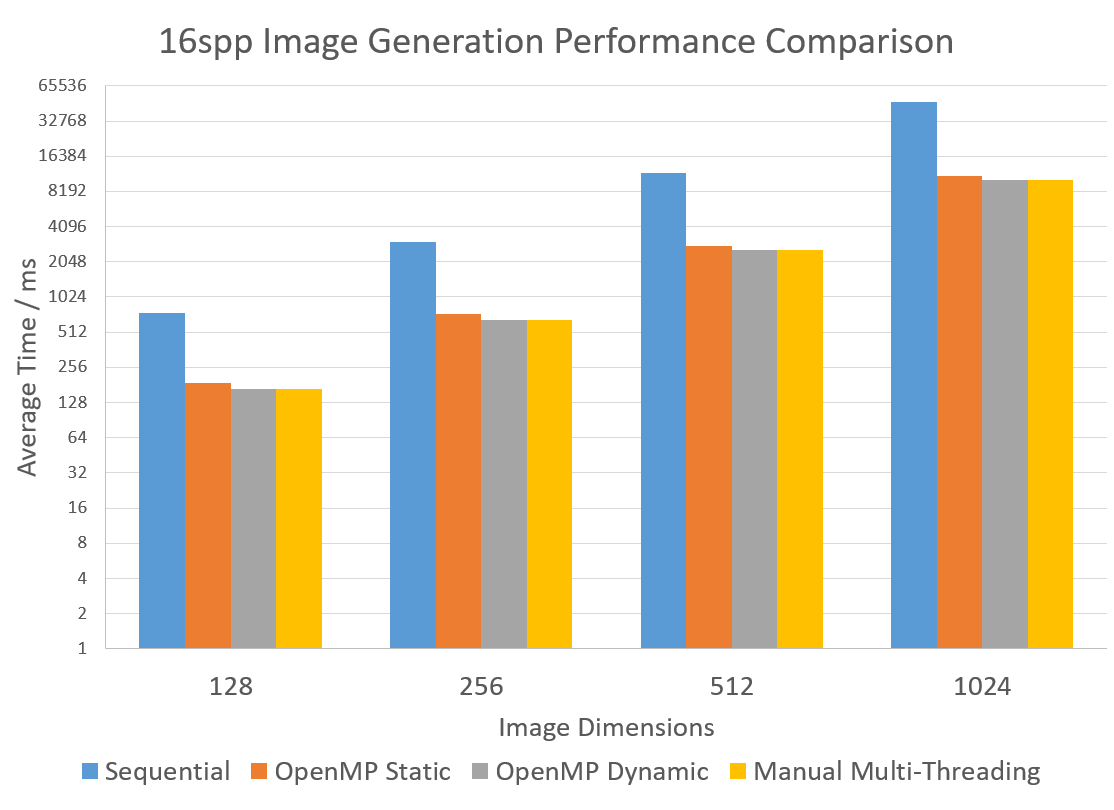
\includegraphics[width=\columnwidth]{IMAGES/performancecomparison2}
		\caption{A graph showing the average time it took each algorithm to generate images of varying dimensions at 16 samples per pixel.}
		\label{graph2}
	\end{figure}

	Once again, the dimensions used for the size of the image were incremented in powers of 2, resulting in a similarly scaled $x$- and $y$-axis, as before. The data from these tests are in line with the previous results. Again it can be seen that the parallel algorithms outperform the sequential algorithm.
	
	There were also a smaller number of tests done at extreme values to compare the algorithm's performances when generating large, high detail images. This is shown in Table \ref{comptable3} below. The data was in agreement with the rest and showed that even at the extreme end the parallelised algorithms generated the images much faster.
	
	\begin{table}[!h]
		\caption{Extreme Spp and Image Size Performance Comparison}
		\label{comptable3}
		\centering
		\resizebox{\columnwidth}{!}{%
			\begin{tabular}{@{}ccccc@{}}
				\toprule
				\multicolumn{5}{c}{Image Dimensions = 1024, Samples Per Pixel = 1024} \\ \midrule
				\multicolumn{1}{c|}{Algorithm} & \multicolumn{1}{c}{Sequential} & \multicolumn{1}{c}{OMP Static} & \multicolumn{1}{c}{OMP Dynamic} & \multicolumn{1}{c}{Manual} \\ \midrule
				\multicolumn{1}{c|}{Test No.} & \multicolumn{4}{c}{Time / ms} \\ \midrule
				\multicolumn{1}{c|}{1} & 3002631 & 709916 & 659067 & 651456 \\
				\multicolumn{1}{c|}{2} & 3001927 & 708573 & 658709 & 647313 \\ \bottomrule
			\end{tabular}%
		}
	\end{table}
	
	By running these averaged times through the formula shown in Equation \ref{efficiencyeq}, the efficiency of these algorithms compared against the sequential algorithm was calculated. The below table (Table \ref{efficiencytable}) shows these efficiencies for the first set of test results.

	\begin{table}[!h]
		\caption{Algorithmic Efficiency Comparison}
		\label{efficiencytable}
		\centering
		\resizebox{\columnwidth}{!}{%
			\begin{tabular}{@{}cccc@{}}
				\toprule
				\multicolumn{4}{c}{Samples Per Pixel = 16} \\ \midrule
				\multicolumn{1}{c|}{Algorithm} & \multicolumn{1}{c}{OMP Static} & \multicolumn{1}{c}{OMP Dynamic} & \multicolumn{1}{c}{Manual} \\ \midrule
				\multicolumn{1}{c|}{Image Dimensions} & \multicolumn{3}{c}{Efficiency} \\ \midrule
				\multicolumn{1}{c|}{128} & 0.997 & 1.125 & 1.108 \\
				\multicolumn{1}{c|}{256} & 1.033 & 1.151 & 1.166 \\
				\multicolumn{1}{c|}{512} & 1.054 & 1.150 & 1.151 \\
				\multicolumn{1}{c|}{1024} & 1.078 & 1.163 & 1.174 \\ \bottomrule
			\end{tabular}%
		}
	\end{table}

	This table shows that some of the algorithms tested had efficiency ratings of more than 1, implying that they ran faster per thread than the sequential algorithm. As stated in the methodology, a few additional tests were done on the parallel algorithms where the number of threads they ran on was controlled. This allowed for a comparison to be made between each algorithm's single threaded performance in order to better contextualise the efficiency ratings of more than 1. Below are two graphs (Figures \ref{graph3} and \ref{graph4}) which show some of the results from these tests.

	\begin{figure}[!h]
		\centering
		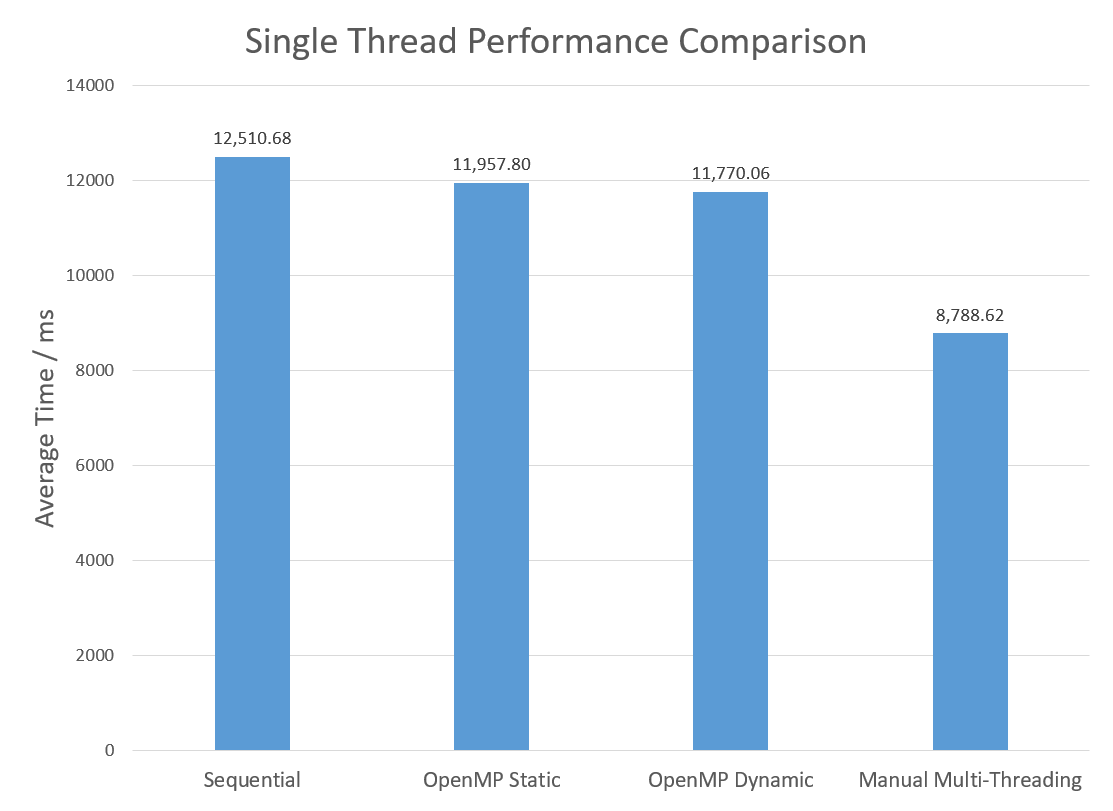
\includegraphics[width=\columnwidth]{IMAGES/singlethreadperformance}
		\caption{A graph showing the average time it took each algorithm to generate a 256x256 image at 16 samples per pixel whilst limited to a single thread.}
		\label{graph3}
	\end{figure}

	Even when ran on a single thread the parallel algorithms generated the required data in less time than the sequential algorithm. In particular, the attempt at manual multi-threading produced significantly faster results. Therefore there were some incidental optimisations of the sequential algorithm when it was parallelised.

	\begin{figure}[!h]
		\centering
		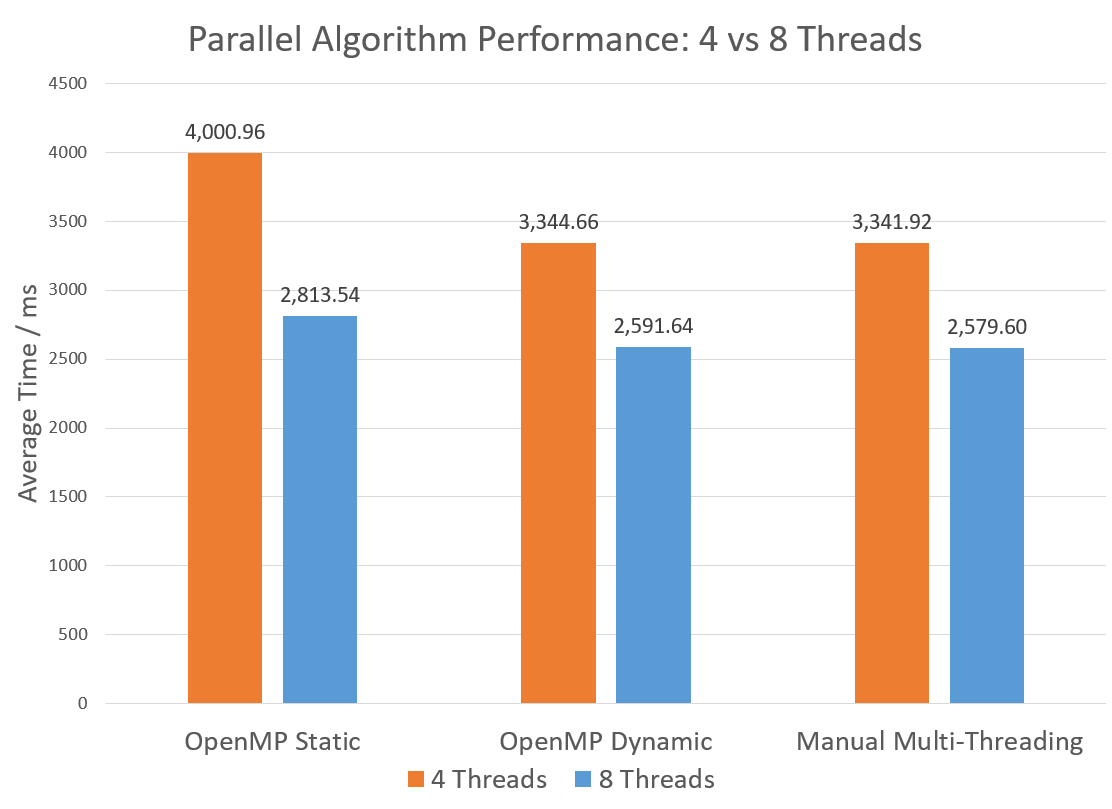
\includegraphics[width=\columnwidth]{IMAGES/threadcomparison}
		\caption{A graph showing the average time it took each algorithm to generate a 256x256 image at 16 samples per pixel on both 4 and 8 threads.}
		\label{graph4}
	\end{figure}

	Further to this, Figure \ref{graph4} shows that there was significant speedup for all the parallelised algorithms when ran on 8 threads instead of 4. The hardware used had 4 cores but allowed for hyper-threading to 8 threads and was potentially a reason for why the efficiencies of more than 1 arose.
	
	\section{Conclusion}
	\subsection{Explanation of Results and Evaluation of Performance}
	Across all the tested algorithms, when either the dimensions of the image or the number of samples per pixel were increased, the time it took to produce the data in the pixel vector used to generate the image would increase with near perfect positive correlation. Furthermore, as shown in Figures \ref{graph1} and \ref{graph2}, independent of whether the image dimensions or the samples per pixels were changed, each of the parallelised algorithms significantly outperformed the sequential algorithm. Compared against each other, OpenMP with static scheduling was always outperformed by both OpenMP with dynamic scheduling	 and the manually multi-threaded algorithm. The manually multi-threading algorithm was generally equal to, or very slightly faster than OpenMP with dynamic scheduling.
	
	Each of the parallelised algorithms had a speedup of 4 or more when compared to the sequential algorithm, and efficiency ratings more than 1. The reasons that the algorithm's efficiency ratings were able to be higher than 1 are likely twofold. Firstly, as shown in Figure \ref{graph3}, the parallelised algorithms were able to generate images quicker than the sequential algorithm even when operating on a single thread. This shows that there were optimisations implemented when parallelising the algorithm, this is especially true for the manually multi-threaded algorithm. Secondly, as shown in Figure \ref{graph4}, there was noticeable speedup from all the algorithms when going from running on 4 threads to running on 8. Given that there were only 4 physical cores and that the equation used to calculate efficiency uses this, a significant proportion of the speedup of the parallelised algorithms is due to the hyper-threading done by the CPU. 
	
	Combined, these two effects make a significant effect on the parallelised algorithm's efficiency ratings. Whilst both parallel algorithms that used OpenMP were only very slightly faster on a single thread than the sequential algorithm, the manually multi-threaded algorithm had a speedup of 1.42 whilst still operating on a single thread. This shows that the performance gained by manually multi-threading the algorithm had much less to do with running the algorithm over multiple threads than the performance gained by the OpenMP parallelised algorithms. The speedup from the hyper-threading, however was more even across the parallelised algorithms.
	
	\subsection{Final Thoughts}
	The provided sequential algorithm originally took a considerable amount of time to produce large images of quality. The attempts at parallelising the algorithm were largely successful. They all performed significantly faster than the sequential algorithm and made the time to generate large images of high detail more manageable. However, whilst running on multiple threads did provide speedup, an important part of the increased performance of the algorithms was due to external optimisations. The attempt at manually multi-threading the algorithm benefited the most from this and as such ended up outperforming both versions of parallelisation using OpenMP. In terms of increased performance purely due to running the algorithm across multiple threads the algorithm that was dynamically scheduled using OpenMP was the top performer.
	
	\bibliographystyle{IEEEtran}
	\bibliography{bibliography}
	
	\newpage
	\onecolumn
	\appendices
	\section{raytracer.cpp}
	\lstinputlisting[caption = The source code for the raytracer.cpp including all the added parallelisation techniques.]{./sourceCode/raytracer.cpp}
	
\end{document}